Este trabalho adota a \emph{Design Science Research} (DSR) como metodologia de pesquisa, uma abordagem focada na concepção, desenvolvimento e avaliação de artefatos tecnológicos para solucionar problemas práticos e relevantes \cite{hevner2004designscienceinformation, dresch2015distinctiveanalysiscase}. O artefato central desenvolvido neste projeto é uma arquitetura de navegação autônoma de baixo custo para robôs de serviço, implementada e avaliada por meio de ambiente de simulação e de um protótipo físico.

Para uma formalização acadêmica, a pesquisa também é classificada conforme a taxonomia de Prodanov e Freitas \cite{prodanov2012metodologiatrabalhocientifico}, detalhada na Seção \ref{sec:Class_Pesquisa}. As etapas práticas do desenvolvimento, alinhadas à DSR, são descritas na Seção \ref{sec:etapas_dsr}.

\section{Classificação da Pesquisa}\label{sec:Class_Pesquisa}

Com base na obra de Prodanov e Freitas \cite{prodanov2012metodologiatrabalhocientifico}, a presente pesquisa é classificada quanto à sua natureza, seus objetivos, seus procedimentos técnicos e à forma de abordagem do problema.

\noindent\textbf{Quanto à Natureza}\par
Do ponto de vista de sua natureza, esta pesquisa classifica-se como \textbf{Pesquisa Aplicada}. Segundo os autores, a pesquisa aplicada ``objetiva gerar conhecimentos para aplicação prática dirigidos à solução de problemas específicos'' \cite[p. 51]{prodanov2012metodologiatrabalhocientifico}. O trabalho se enquadra nesta definição, pois busca desenvolver e avaliar uma solução tecnológica (artefato) para resolver problemas práticos e imediatos: a navegação confiável de robôs de serviço em ambientes dinâmicos e as restrições de custo em hardware com recursos limitados.

\noindent\textbf{Quanto aos Objetivos}\par
No que se refere aos seus objetivos, a pesquisa combina características de três tipos: \textbf{Exploratória}, \textbf{Descritiva} e \textbf{Explicativa}.
\begin{itemize}
    \item \textbf{Pesquisa Exploratória:} Na fase inicial, o trabalho possui um caráter exploratório, que, segundo \citet[p. 51]{prodanov2012metodologiatrabalhocientifico}, ``tem como finalidade proporcionar mais informações sobre o assunto que vamos investigar''. Isso se evidencia no Objetivo Específico 1, que prevê a realização de uma revisão da literatura sobre algoritmos de vSLAM para fundamentar as decisões de projeto.
    \item \textbf{Pesquisa Descritiva:} A pesquisa assume um viés descritivo na fase de validação, pois visa ``descrever as características de determinada população ou fenômeno'' \cite[p. 52]{prodanov2012metodologiatrabalhocientifico}. Isso ocorre na mensuração de métricas de desempenho computacional (consumo de CPU e memória) e de qualidade da navegação (precisão do mapeamento), conforme detalhado no Objetivo Específico 3.
    \item \textbf{Pesquisa Explicativa:} Por fim, o trabalho almeja alcançar um nível explicativo, que ``visa a identificar os fatores que determinam ou contribuem para a ocorrência dos fenômenos'' \cite[p. 53]{prodanov2012metodologiatrabalhocientifico}. A questão de pesquisa busca explicar se a arquitetura proposta (fator determinante) é tecnicamente viável para alcançar um desempenho funcional (fenômeno), estabelecendo uma relação de causa e efeito entre a solução e os resultados.
\end{itemize}

\noindent\textbf{Quanto aos Procedimentos Técnicos}\par
Considerando os procedimentos técnicos, esta pesquisa classifica-se como \textbf{Pesquisa Bibliográfica} e \textbf{Pesquisa Experimental}.
\begin{itemize}
    \item \textbf{Pesquisa Bibliográfica:} É desenvolvida ``a partir de material já publicado'' \cite[p. 54]{prodanov2012metodologiatrabalhocientifico}, sendo fundamental para a primeira etapa do trabalho, conforme descrito na metodologia.
    \item \textbf{Pesquisa Experimental:} É o procedimento central do trabalho, pois ``selecionamos as variáveis que seriam capazes de influenciá-lo, definimos as formas de controle e de observação dos efeitos que a variável produz no objeto'' \cite[p. 57]{prodanov2012metodologiatrabalhocientifico}. O objeto de estudo é o desempenho da navegação, e a validação é conduzida em cenários de teste controlados (simulados e físicos) para observar e mensurar os efeitos da arquitetura implementada.
\end{itemize}

\noindent\textbf{Quanto à Forma de Abordagem do Problema}\par
A abordagem do problema é predominantemente \textbf{Quantitativa}, com elementos de análise \textbf{Qualitativa}.
\begin{itemize}
    \item \textbf{Pesquisa Quantitativa:} A abordagem quantitativa ``considera que tudo pode ser quantificável, o que significa traduzir em números opiniões e informações para classificá-las e analisá-las'' \cite[p. 69]{prodanov2012metodologiatrabalhocientifico}. A validação do projeto reside na coleta e análise de dados numéricos objetivos, como consumo de CPU, memória, acurácia do mapa e eficiência da navegação.
    \item \textbf{Pesquisa Qualitativa:} A abordagem qualitativa, que foca na ``interpretação dos fenômenos e a atribuição de significados'' \cite[p. 70]{prodanov2012metodologiatrabalhocientifico}, é empregada de forma complementar na análise dos resultados, especialmente para interpretar as causas de falhas ou comportamentos inesperados durante os testes de desvio de obstáculos dinâmicos, que são mais difíceis de quantificar puramente.
\end{itemize}

\section{Etapas da Pesquisa (DSR)}
\label{sec:etapas_dsr}

Enquanto a Seção \ref{sec:Class_Pesquisa} classificou a pesquisa de forma taxonômica, esta seção detalha o processo metodológico prático. Este trabalho é conduzido pela \emph{Design Science Research} (DSR) \cite{hevner2004designscienceinformation, dresch2015distinctiveanalysiscase}, uma metodologia focada na concepção, construção e avaliação de um artefato tecnológico para solucionar um problema prático.

O problema prático, conforme definido na Introdução, é a dificuldade de executar algoritmos de vSLAM em plataformas robóticas de baixo custo e com recursos computacionais limitados \cite{costa2019characterizingpolybenchgpu, li2021highefficientmultirobot}. O artefato a ser desenvolvido e avaliado é, portanto, uma \textbf{arquitetura de navegação autônoma funcional}, que integra hardware de baixo custo (um Raspberry Pi e uma câmera RGB-D) e um \emph{stack} de software (ROS e algoritmos de vSLAM/Navegação) capaz de operar sob essas restrições, seja via otimização local ou processamento distribuído.

O processo de DSR será executado em três etapas iterativas. A Figura \ref{fig:fluxo_metodologia} ilustra o fluxo metodológico adotado, detalhando as atividades específicas de cada fase e o ciclo de realimentação (feedback) entre a validação e a fundamentação teórica.

\begin{figure}[H]
    \centering
    \caption{Fluxograma das etapas da metodologia DSR aplicadas ao projeto}
    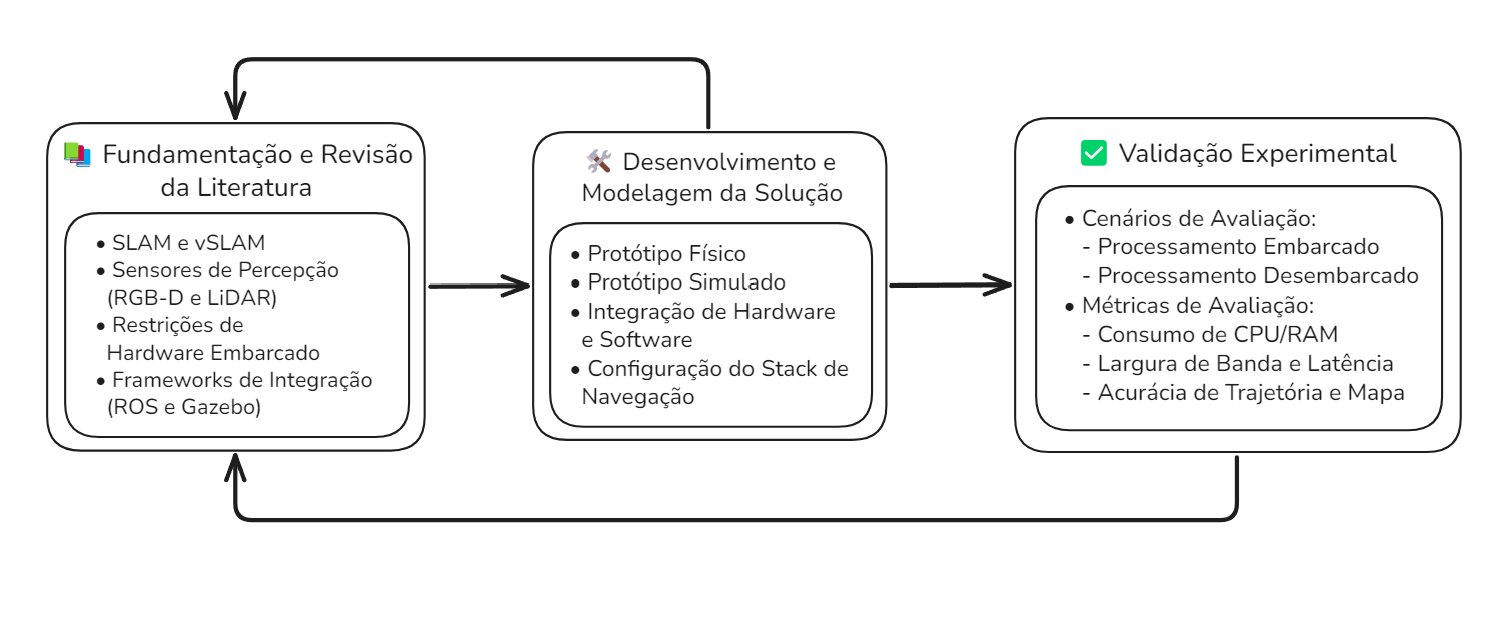
\includegraphics[width=1.0\textwidth]{figuras/fluxoDSR.png}
    \label{fig:fluxo_metodologia}
    Elaborado pelo autor (2025).
\end{figure}

As etapas ilustradas são descritas detalhadamente nas subseções a seguir.

\subsection{Etapa 1: Fundamentação e Revisão da Literatura}
\label{ssec:etapa1_revisao}

A primeira etapa consiste na investigação teórica para identificar a lacuna de pesquisa e fundamentar as decisões de projeto do artefato. Esta revisão abrange quatro pilares centrais:

\begin{enumerate}
     \item \textbf{SLAM e vSLAM:} Estudo dos fundamentos teóricos do SLAM e sua evolução para o vSLAM (Visual SLAM). O foco é entender como algoritmos utilizam sensores visuais para realizar o mapeamento e a localização \cite{taheri2021slamdefinitionevolution, guapacha2017localizacaomapeamentosimultaneos}, bem como estratégias para converter dados de profundidade em varreduras 2D para otimização de desempenho \cite{zhang2023rgbdnavigation2d}.
    
    \item \textbf{Sensores de Percepção (RGB-D):} Análise de câmeras RGB-D (como o Kinect) como sensores primários de percepção. Esta investigação compara suas vantagens e desvantagens em relação a sensores LiDAR, analisando métodos para mitigar o campo de visão limitado e melhorar a precisão do mapa através da fusão sensorial \cite{kamarudin2015improvingperformance2d}.
    
    \item \textbf{Hardware Embarcado:} Investigação dos desafios de implementar vSLAM em \textit{Single Board Computer} (SBC) de baixo custo, como o Raspberry Pi \cite{raspberrypi2019raspberrypi}. A análise foca nos gargalos computacionais (consumo de CPU e memória) gerados pelo processamento intenso de imagens, extração de características (como ORB e BRIEF) e otimização de grafos.
    
    \item \textbf{Frameworks de Integração (ROS e Gazebo):} Estudo do \emph{Robot Operating System} (ROS) como \emph{middleware} padrão para o desenvolvimento de robôs complexos. Além disso, será investigado o uso do simulador \textbf{Gazebo} como ferramenta de prototipação virtual, essencial para validar a lógica de navegação e os algoritmos de SLAM antes de sua implementação no hardware físico.
\end{enumerate}

\subsection{Etapa 2: Desenvolvimento e Modelagem da Solução (O Artefato)}
\label{ssec:etapa2_artefato}

Esta etapa constitui o núcleo da pesquisa (a ser detalhado no Capítulo \ref{cap-desenvolvimento}) e foca na construção e integração do artefato. Para mitigar riscos e validar a arquitetura de forma incremental, será utilizada uma abordagem de \textbf{prototipação dual}: um protótipo simulado e um protótipo físico.

Será desenvolvido um modelo de simulação 3D do robô e do ambiente de teste. O simulador \textbf{Gazebo} \cite{koenig2004designuseparadigms} será utilizado para criar um ``gêmeo digital'' do hardware, permitindo a validação da lógica de controle e do \emph{stack} de vSLAM em um ambiente controlado, realista e repetível. Esta etapa envolverá:
\begin{itemize}
    \item A modelagem do robô em formato URDF (\emph{Unified Robot Description Format}), descrevendo sua geometria, física e juntas (\textit{joints}).
    \item A configuração de \emph{plugins} de simulação para os sensores, notadamente a câmera RGB-D e a unidade de medição inercial (\textbf{IMU}), garantindo que os fluxos de dados gerados no ROS sejam compatíveis com os do hardware real.
\end{itemize}

Paralelamente, será construído o protótipo físico, que servirá como plataforma de validação final. A construção seguirá os princípios de baixo custo e modularidade identificados na Etapa 1. As fases de desenvolvimento são:

\begin{itemize}
    \item \textbf{Montagem e Integração de Hardware:} O chassi do robô móvel será equipado com (i) a unidade de processamento central (Raspberry Pi), (ii) os atuadores (motores e drivers de ponte H) e (iii) os sensores de percepção e odometria (câmera RGB-D, unidade de medição inercial - IMU).
    
    \item \textbf{Desenvolvimento do Firmware de Baixo Nível:} Um microcontrolador (como a plataforma Arduino) será programado para atuar como um controlador de baixo nível. Este firmware será responsável por receber comandos de velocidade (ex: PWM para as pontes H) e ler os dados brutos do sensor IMU, disponibilizando-os para o Raspberry Pi via comunicação serial.
    
    \item \textbf{Desenvolvimento do Software Embarcado (ROS 2):} No Raspberry Pi, um ambiente ROS 2 será configurado para orquestrar o sistema. O desenvolvimento de software focará na integração dos drivers de percepção (câmera RGB-D e IMU) e na interface de comunicação com o microcontrolador para o controle dos atuadores. Adicionalmente, serão implementadas as configurações necessárias para a conversão de dados de profundidade em varreduras 2D \cite{zhang2023rgbdnavigation2d} e a execução dos algoritmos de SLAM selecionados, permitindo a alternância flexível entre as estratégias de processamento local otimizado e distribuído.
\end{itemize}

\subsection{Etapa 3: Validação Experimental}
\label{ssec:etapa3_validacao}

A etapa final consiste na execução de experimentos controlados para avaliar o desempenho do artefato e responder à questão de pesquisa. A validação será conduzida nos ambientes simulado e físico, focando na principal restrição do projeto: o recurso computacional limitado e a largura de banda de rede.

O principal eixo de experimentação será a comparação de desempenho entre duas estratégias de processamento arquiteturais:

\begin{enumerate}
    \item \textbf{Processamento Embarcado (\emph{Onboard}):} O algoritmo de SLAM e todos os nós ROS serão executados inteiramente dentro do Raspberry Pi. Este cenário representa a arquitetura de robô totalmente autônoma e de menor custo. Serão avaliados tanto o desempenho de algoritmos vSLAM 3D densos quanto a viabilidade de algoritmos 2D otimizados via simulação de laser visual \cite{kamarudin2015improvingperformance2d, zhang2023rgbdnavigation2d}, buscando o limite operacional do hardware.
    
    \item \textbf{Processamento Desembarcado (\emph{Offboard}):} O Raspberry Pi atuará apenas como um ``coletor de sensores'', utilizando sua capacidade de CPU para capturar os dados da câmera RGB-D e da IMU, transmitindo-os via rede sem fio (Wi-Fi). O processamento computacionalmente intensivo do vSLAM será executado em uma estação de trabalho (PC/Desktop) mais potente. Esta abordagem simula uma arquitetura de \emph{cloud robotics} ou \emph{computing offloading}.
\end{enumerate}

Para avaliar o desempenho da arquitetura proposta, serão coletadas métricas computacionais e de qualidade da localização/mapeamento. Além das métricas quantitativas, será realizada avaliação qualitativa do mapa gerado (inspeção de completude e coerência).
\begin{itemize}
    \item \textbf{Métricas de Desempenho Computacional:} Uso de CPU, memória RAM, taxa de quadros por segundo (FPS), latência média por etapa e estabilidade (variação ao longo do tempo, incluindo efeitos de \emph{thermal throttling});
    \item \textbf{Métricas de Comunicação de Rede (Offboard):} Latência e \emph{jitter}, perda de pacotes e \emph{throughput}, avaliando a influência da rede na robustez do sistema;
    \item \textbf{Métricas de Qualidade do SLAM (Resultado):} Métricas de trajetória/localização, como ATE (\textit{Absolute Trajectory Error}) e RPE (\textit{Relative Pose Error}) quando houver referência disponível, taxa de perda de rastreamento/perda de pose e qualidade do mapa (completude e consistência visual).
\end{itemize}

A análise comparativa dessas métricas permitirá concluir sobre a viabilidade técnica da arquitetura proposta para robôs de serviço domésticos.